\section{Research Plan}

Figure \ref{fig:flow} shows the basic outline of a proposed workflow
and components needed to support feedback-driven mutation testing.
These components serve to organize the research plan.

\subsection{Mutant Generator}
\label{sec:anylangplan}

The most widely-used mutation testing tool in the real world
is PIT~\cite{pittest}, which targets Java bytecode.  There are recent attempts
to provide the same kind of support for other languages, especially C, by
targeting LLVM IR~\cite{HaririLLVM}.  This poses several problems for
feedback-driven mutation testing. 
First, bytecode- or IR-level mutation works well to compute a
score for a test suite, but is not not suitable for presentation to developers
or test engineers, who need to reason about a mutant's implications for their
source or test code.   That is, Java developers
think in terms of Java, not compiled bytecode; C and C+++ developers certainly
do not generally understand LLVM IR; test engineers are even less likely to
appreciate such low-level descriptions.  Even when possible, translation may not help: a bytecode-level
mutation may not have a simple source-level equivalent, especially if the
bytecode has been optimized.  Second, features that help identify semantically
similar (or dissimilar) mutants are hard to identify at the bytecode level.  Even if the mutant
is, for example, a constant replacement in one case and an arithmetic operator
replacement in another, the fact that both take place inside an argument to a
logging function with an {\tt INFO} argument may be enough to predict that their
effects are redundant.
Finally, IR-specific tools are by construction limited to their associated
language ecosystems, excluding a large body of code written in other languages,
as well as project-specific DSLs.
Moreover, the vast majority of software projects are written
in multiple languages~\cite{Ray2014}.  Our desire for real-world applicability
thus motivates polyglot analysis and testing infrastructure.  

Thus, our first research task is to develop a novel {\tt mutant generator} that
(1) operates at the source level, with output that is easy for developers to
understand and the framework to analyze; (2) is, as much as possible,
\emph{language independent}, and applicable to projects written in a
heterogeneity of languages; and finally (3) is efficient.  The PI's recent
advances in universal mutation~\cite{regexpMut,universalmutator} and
language-agnostic declarative program transformation using parser
combinators~\cite{rvt-ppcs} provide key motivation and starting points for this
component.

\subsubsection{Background and preliminary work}

% CLG: I'm tempted to cut some of the universal mutator content.  I view it as
% important in that it shows that language-agnostic, syntax-driven mutation is
% viable for mutation testing, but since we're mostly building on Comby here, we
% need the space for that

\begin{figure}
\begin{tabularx}{0.75\textwidth}{XXX}
\verb|\+ ==> -| & \verb|== ==> !=| & \verb|(\D)(\d+)(\D) ==> \1(\2+1)\3|\\
\verb|\+ ==> *| & \verb|== ==> <| & \verb|(\D)(\d+)(\D) ==> \1(\2-1)\3|\\
\verb|\+ ==> /| & \verb|== ==> >| & \verb|(\D)(\d+)(\D) ==> \g<1>0\3|\\
\verb|".+" ==> ""| & \verb|while ==> if| & \verb|(^\s*)(\S+.*)\n ==> \1\2\n\1break;\n|\\
%{\tt \\+ ==> *} & {\tt != ==> <=} & {\tt (\D)(\\d+)(\D) ==> \\1\\2-1\\3}\\
%{\tt \\+ ==> /} & {\tt != ==> >=} & {\tt ".+" ==> ""}\\
%{\tt \\+ ==> \%} & {\tt != ==> >=} & {\tt (^\\s*)(\\S+.*)\\n ==> \\1\\2\\n\\1break;\\n}\\
\end{tabularx}
\caption{Some universal mutation rules}
\label{fig:rules}
\end{figure}

The PI's combined prior work provides two important pieces of evidence for the
feasibility of Any-Language mutation.  

\paragraph{The universalmutator.} First, PI Groce and colleagues
released a functional, regular-expression-based mutant
generator~\cite{regexpMut,universalmutator}.
This {\tt universalmutator} 
does not attempt to parse source code, but simply defines mutation
operators by a set of regular-expression-defined text transformations.  These
are organized into a hierarchy, so that if a program is, e.g., written in Swift,
the ``universal'' mutation operators that apply to all programming languages are
first applied, then operators for ``C-like'' languages, and finally a set of
Swift-specific rules are applied.  Figure \ref{fig:rules} shows some of the
current set of ``universal'' rules applied to all languages.  

Importantly,  PI Groce demonstrated that the {\tt universalmutator} tool generated
numbers of mutants and kill ratios for Java code comparable to
PIT~\cite{pittest} and Major~\cite{Major}.  For falsification-driven
verification, the regular-expression-based approach produced mutants of equal
value to those produced by Andrews' tool~\cite{mutant} and Muupi~\cite{muupi}
for C and Python, respectively.  
%
% As it stands, the {\tt universalmutator} tool
% is usable for real-world mutation (in fact, it is being considered for use by
% NASA/JPL engineers in testing the C code for upcoming CubeSat~\cite{CubeSat}
% missions) for languages including: C, C++, Java, Python, Swift, Rust, Go, and
% the Solidity smart-contract language.  The {\tt universalmutator} allows easy
% definition of new rules, and supports automated analysis of mutants,
% coverage-based pruning of mutants, and (in some languages) trivial compiler
% equivalence~\cite{TCE} checks.
%
% Adding a new
% language, even a custom DSL, or a new set of project-specific rules for an
% existing language, in this approach, simply requires writing a new rule file and
% defining where it lies in the language hierarchy.  In our feedback-driven
% setting, the problem of generating ``too many'' mutants is irrelevant: only a
% small set of highly diverse and likely-actionable mutants is ever presented to
% the
% user. %, and a novelty-estimator helps a user stop examining new mutants when the payoff is likely to be low.
%
% TODO: probably cut back on this stuff.
This preliminary work demonstrates that multi-language, syntax-driven, source-level mutation is
feasible and, indeed, effective, producing results competitive with
state-of-the-art single-language mutation tools.  
However, it has significant limitations for long-term utility, motivating the
propsoed research below: Because the source
code is not parsed, and applies the regular expressions to lines of code, not
larger blocks, the technique generates many mutants that are not valid programs,
and cannot be compiled, or that are trivially equivalent because they, e.g.,
mutate ``source code'' in a large comment block.  Integrating mutation
generation with execution is currently supported, but extending it to new
languages or build systems is hard for users, requiring writing considerable
Python code or complex shell scripts.  
%It is currently impossible to define
%mutation operators that apply to blocks of code rather than text within a single
%line, and standard regular expressions are not really suited to describing code
%constructs such as blocks, functions, classes, or structs.  Natural formatting
%of, e.g., an s-expression in a LISP-family language can hide opportunities for
%mutation, such as switching argument orders.  
Fundamentally, regular expressions are
only occasionally a natural notation for expressing source-level mutation;
source in all languages differs from arbitrary unstructured strings.

\paragraph{Comby: Declarative, any-language transformation.} Fortunately, recent work by PI
Le Goues and collaborators introduced a powerful new representation to
declaratively 
transform richer syntactic structures in programs across multiple
languages~\cite{rvt-ppc}. \textbf{FIXME: 2--3 sentences on how it works: what's
  the key magic?  Words like ``parser combinators'' would be useful; the idea is
to talk about how we get parsing without needing a parse tree.  This is the key
magic, and we need to sell it; recall the reviewers who don't believe how good
it is...it may be preferable to pull out some of the content currently in the
next subsub section on proposed work up to here, and focus the proposed work on
improvements Comby needs to be even more awesome for mut testing (LSPs, whatever
else).}  This work has
already shown its practical utility by
performing lightweight refactors in more than 10 languages (including those
targeted by {\tt universalmutator}). The associated tool, {\tt
comby}~\cite{comby-github}, enables a new language-general way of expressing
transformations that regular expressions cannot typically recognize (e.g.,
nested code blocks). \textbf{FIXME: 2--3 sentences summarizing results (esp efficient,
  expressive power)} 
%Current mutation testing approaches largely rely on either
%sophisticated language-specific tools that fail to generalize to other
%languages~\cite{Major} or rudimentary textual manipulation~\cite{mutant} that is
%fundamentally limited in effectiveness.
Coupling declarative syntax manipulation that goes beyond the limits
of regular expressions with
mutation testing promises to yield greater effectiveness by (a) targeting more
sophisticated properties of programs, and (b) delivering more user-accessible
tools for developing mutation transformations. Our already achieved advances in 
real-world tooling (i.e., in {\tt universalmutator} and {\tt comby}) suggest that
this goal is imminently feasible.  At heart, this line of work
represents the conviction of the PIs that mutation testing (like
automated program repair) is simply
an instance of the general field of automated program transformation~\cite{Ptransform}.

\subsubsection{Proposed work: Any language mutation}

Our goal is a source-level mutant generator that can apply to any language,
maximizing applicability and usability.  
 The {\tt
  universalmutator} provides an initial source of mutants that
satisfies this requirement for initial experimentation, but for
long-term effectiveness is both inefficient and inexpressive.  


% The source of all mutants to be presented to the user is the mutant
% generator, and in order to maximize the effectiveness of the approach,
% this proposal aims to allow effective generation of mutants for any
% programming
% language or DSL, with minimal additional effort. The
% current implementation avoids parsing to such an extent that it
% generates numerous useless mutants embedded in code comments, or that
% are obviously syntactically invalid.  While avoiding a parser-based
% approach, simple additional constraints could avoid this, without
% adding burden on users, such as allowing the definition of a
% language's comment mechanisms, and not producing mutants inside
% comments.  More generally, a mechanism for disabling mutation in
% contexts defined in the same way as mutation operators would handle
% other, even project-specific, constraints (e.g., never mutate inline
% assembly in C/C++).  A problem with the current representation of
% mutation operators and such contexts is that regular expressions are
% currently applied only at the line level, and in any case are not
% effective for defining such fundamentally non-regular aspects of code
% as blocks and nested delimiters.  A key goal in this project is to greatly
% enhance
% % the regular-expression language (without losing its simplicity
% %for ``normal'' operators) with the ability to express, in a
% %language-independent, syntactic form, such context-dependent aspects
% %of code.
% the expressity of transformations (e.g., operators for multi-line, context-dependent program fragments) while retaining the simplicity of specifying usual % or "normal" operators as above, but I'm not sure what normal is? Is Fig. 1 representative?
% operators.

We therefore propose to use {\tt comby}~\cite{comby-github, rvt-ppc} for specifying
transformations and generating mutants. {\tt Comby} uses
declarative templates that describe before/after changes for program fragments. For example, the following transformation swaps the first two arguments of the function {\tt memcpy}:

\begin{figure}[!h]
\centering
\begin{BVerbatim}[commandchars=\\\{\}]
memcpy(\textcolor{blue}{:[1]}, \textcolor{ForestGreen}{:[2]}, :[3]) ==> memcpy(\textcolor{ForestGreen}{:[2]}, \textcolor{blue}{:[1]}, :[3])
\end{BVerbatim}
\end{figure}

Hole syntax \verb|:[1]| binds syntax to a variable. A unique property of {\tt
  comby} templates is that variables
\emph{only} bind to syntax that occurs
inside well-balanced delimiters (like parentheses), whitespace is handled intelligently, %(i.e., a space indicates any whitespace, including newlines)
and syntax otherwise matches literally. % (i.e., with minimal metasyntax).
Concretely, this means that the template above seamlessly transforms syntax structure in complex fragments as in the following:

\begin{figure}[!h]
\footnotesize
\begin{subfigure}[t]{.47\textwidth}
\centering
\begin{Verbatim}[commandchars=\\\{\}]
memcpy(\textcolor{blue}{*stream->main_data + stream->md_len},
       \textcolor{ForestGreen}{mad_bit_nextbyte(&stream->ptr)},
       frame_used = md_len - si.main_data_begin);
\end{Verbatim}
\end{subfigure}%
\begin{subfigure}[t]{.04\textwidth}
\begin{verbatim}

==>

\end{verbatim}
\end{subfigure}%
\begin{subfigure}[t]{.47\textwidth}
\begin{Verbatim}[commandchars=\\\{\}]
memcpy(\textcolor{ForestGreen}{mad_bit_nextbyte(&stream->ptr)},
       \textcolor{blue}{*stream->foo_data + stream->md_len},
       frame_used = md_len - si.foo_data_begin);
\end{Verbatim}
\end{subfigure}
\normalsize
\end{figure}
% The above fragment comes from real example: https://sourcegraph.com/github.com/markjeee/libmad/-/blob/layer3.c#L2637
% The above example of in a live example here: bit.ly/2Nmh3v2

At a high-level, {\tt comby} performs
% actual
context-free
parsing of syntactic structures that typically correspond to nested expressions and blocks in the underlying AST.\footnote{Regular expressions are not powerful enough to recognize such program terms in the general case.} Templates offer a \emph{declarative} description for matching and rewriting these structures in a way that is syntactically close to the source code.
In addition, {\tt comby} can distinguish between code, strings, and comments. Templates contextually matches or ignores these dimensions of a program. % (which are common to virtually all languages)
% Compared to regular-expressions, {\tt comby} can match on nested structures, can discriminate between code, data (strings), and comments on a language-aware basis.
{\tt Comby} is language-aware in the sense that small language definitions describe whether syntax should be balanced (e.g., parentheses or braces) or delineate strings or comments. These definitions describe a coarse structural decomposition of programs (as typically understood by compilers) rather than just a sequence of characters (as treated by regex). Language definitions already exist for 20+ languages, and supports a simple extension mechanism for new languages (e.g., Solidity) or custom DSLs.\footnote{\url{https://comby.dev/\#faq-language-support}}

We believe that accessible structural syntax manipulation can achieve a leap in
expressivity and effectiveness for mutation testing. % a cite to substantiate "based on what" would be nice
For one, targeted structural and contextual changes are
more likely to produce a well-formed syntactic programs
% compared to the regex counterpart
that exercise interesting paths in a test suite.
We propose to extend {\tt universalmutator}
to generate mutants from {\tt comby} templates, and to evaluate the efficacy of
% truly
multi-language mutation testing with structural code changes. % for the first time, no?
\textbf{FIXME: propose the LSP work to pull in type/static information.  A
  reviewer who knows our work might say ``what's the new research, here?''
  (indeed, a reviewer did say that about universalmutator).  Sometimes it's fine
  to just be like, there is no new research, but we'll use this thing for this
  part...but given that we HAVE new research to do, it's worth proposing it.}

%the Cobra code-checking tool's language~\cite{Cobra} is an
%example of the kind of approach desired, though the language itself
%must be different, since transformation,
%not just detection, is the expressive content of a mutation operator.
The generator will also need to be improved to allow users
to easily specify novel build environments and plug-ins for checking
Trivial Compiler Equivalence~\cite{TCE} to make the entire
feedback-driven mutation process workable.  \textbf{FIXME, rvt: can we keep this
  and think about making it work for comby?} Because some distance
metrics may require compiling mutants, which is costly, a specialized
projection of the distance only requiring textual analysis will need
to be developed, to allow generation, compilation, and execution of
only high-priority mutants for very large projects.

% FIXME: integrate me in here somewhere, as a benefit.
\textbf{FIXME: RVT: this paragraph speaks to the benefit of avoiding parsing;
  perhaps you can integrate the idea into the Comby text you add? And then cut this?} 
One ongoing limitation of mutation testing is that tools are often research
projects, and eventually become unusable due to lack of support, even in
mainstream languages such as Java and C~\cite{MutChoice}.
This is because mutation tools that parse a language and guarantee generation of
valid programs in the source language are complex, hard-to-maintain-and-extend
systems; language complexity makes such a tool for C++, for example, an
extremely daunting task.   

\subsection{FPF-Based Novelty Ranking}
\label{sec:fpfplan}

\begin{figure}[t]
\centering
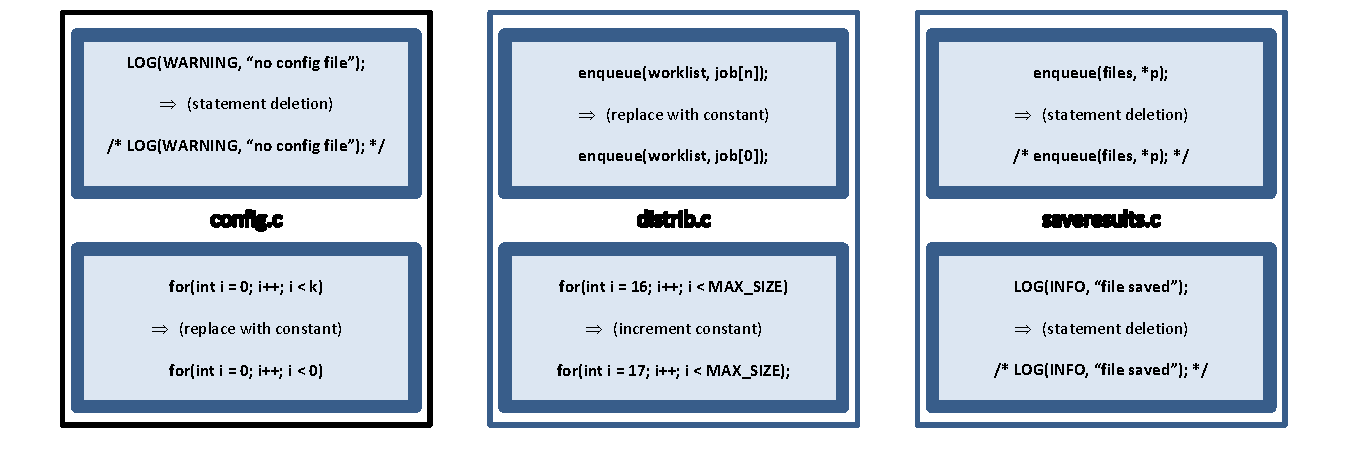
\includegraphics[width=0.95\columnwidth]{distmetric}

\caption{Which mutants are most similar?  If the user marked the
  mutant in the upper left corner as uninteresting and added a test
  to kill the
  mutant in the upper middle, which mutant
  should she examine next?}
\label{fig:distances}
\end{figure}


Our vision of feedback-driven mutation testing is predicated on selecting and ranking a small
set of highly interesting mutants to present to the developers.  An unkilled
mutant is, conceptually, very similar to a failing test.  It presents
information of possible relevance to a developer.  The mutant or test \emph{may}
indicate the presence of a previously unknown fault that needs to be fixed,
either in the SUT or in testing.  It may indicate the presence of a previously
unknown fault of less importance.  It may also indicate an even less interesting
result: an equivalent mutant or an inherently flaky test.  Additionally, an
unkilled mutant or failing test may contain information that is uninteresting
because \emph{it duplicates information already examined.}  While examining an
equivalent mutant is not always useless (e.g., it may indicate an opportunity
for refactoring or improving the efficiency of
code~\cite{ivankovic2018industrial,groce2018verified}), examining a mutant that
is equivalent to, or extremely similar to, an already-understood mutant is
almost never worthwhile.  A key research challenge is thus to select and
prioritzize mutants that provide maximum utility to a user.  

Current mutation testing approaches make little effort (with a few exceptions~\cite{MutGoogle,FaRM})
to prioritize mutants.  Other than (arguably) some efforts to
incorporate dominance results~\cite{MutQuality}, no mutation testing approaches
currently suggest any more sophisticated way to maximize the novelty of
presented mutants than stratified sampling~\cite{gopinath2017mutation};
stratified sampling does not aim at semantic novelty, and can present many
mutants from the same class, if applied at the method level, even if those
mutants are highly similar in impact.  Other work~\cite{gopinath2015howhard}
proposes random sampling as the most effective way to select mutants.
Unfortunately, when an important class of unkilled mutants has only a few
members, random sampling is almost guaranteed to fail to present any of them.  
Our preliminary results argue, however, that novelty-based clustering is a
promising approach for solving this problem. 

\subsubsection{Background and preliminary work} 

The mutant selection and prioritization problem is analogous to a similar
problem in fuzz testing and triage.  That is, instead of contending with a large
list of undifferentiated inputs (or mutants), a user ideally preferes a few,
most important, or most-critical inputs, that maximize the amount of payoff in
terms of bugs found or information gained.

\paragraph{Furthest point first and fuzzer taming} Fuzzer taming~\cite{PLDI13}
was a solution PI Groce and colleagues proposed to the problem 
of triaging test failures in automated test generation~\cite{SemCrash}.  
Like mutant generators, fuzzers tend to produce very large numbers of failing
tests (mutants) for a much
smaller number of distinct bugs (interesting behaviors).  Finding the set of distinct bugs,
and identifying important bugs that need to be fixed immediately is
difficult, because the important bugs may be represented by only one
or two failing tests in a set of thousands of failing tests, most of
which are duplicates.  The fuzzer taming work proposed that rather than highly imprecise
clustering, which does not work well in practice, and handles outliers
in a way that does not match the ``power law'' distribution of bugs, an
algorithm matching the goal of ranking maximally-different test
failures highly was appropriate. 

The \emph{furthest-point-first} (FPF) algorithm of
Gonzalez~\cite{Gonzalez85} does precisely this.  FPF, beginning with
any randomly chosen test (or mutant, in the present setting), always ranks
next the point in a metric-defined space that has the \emph{greatest
  distance from the previously ranked point to which it is closest.}
That is, for each point (test or mutant) not yet presented to the
user, FPF finds the closest among all already-ranked points, and
associates each unranked point with the distance to that closest
point.  The unranked point with the largest such distance is then
added to the ranking, and the process is repeated.  FPF can be
computed by a greedy algorithm, and is known to approximate novel-item
discovery for an optimal clustering~\cite{Gonzalez85}.  Preliminary work on the fuzzer taming problem using FPF-based
techniques~\cite{PLDI13,distMut} can be directly applied
to the different problem of ranking
unkilled mutants such that novel mutants are presented first.  %The
%research plan (Section
%\ref{sec:fpfplan}), discusses the key \emph{differences} between novelty ranking
%for mutants and
%the fuzzer taming problem.

\paragraph{Preliminary use of FPF-based mutant ranking.} In collaboration with security analysts at Trail of Bits, PI Groce
implemented a prototype version of mutant priorization, without
feedback, using a manually constructed distance metric tailored to
Solidity smart contracts.  This was an essential step in an effort to
use mutation analysis to compare three static analysis tools for smart
contracts~\cite{slitherpaper,sc:smartcheck,securify}.  The comparison of three such tools over 100 random contracts
from the Ethereum blockchain~\cite{buterin2013whitepaper,wood2014yellow} required analysis of 46,769 mutants, with
46,752 of these not killed by at least one static analysis tool.  The
aim of the analyis was to 1) find cases where mutation caused each
tool to flag a \emph{new} issue with the source code (thus
differentially identifying kills), then 2) find cases where at
least one tool flags a mutant, while others do not, and finally 3) baseline
this with respect to general warning rates for the tools over the same contracts.
Sorting through the surviving mutants to understand weaknesses of the
tools was simply not possible without using a simple version of the
FPF ranking algorithm, combined with an \emph{ad hoc} distance
metric.  With even this rudimentary, untuned version of our approach,
PI Groce and Trail of Bits engineers identified three significant new
detectors, which were implemented and added to the Slither static
analysis tool~\cite{slitherpaper}.  These are currently in use by Trail of Bits for
security audits, and will be released to the public after tuning.  Without the FPF ranking, finding these three
opportunities for improving Slither would not have been feasible.  To
our knowledge, the use of mutation to compare and improve static
analysis tools, rather than test suites, in this \emph{differential}
(both within tools and across tools) sense, is novel, and we believe that
feedback-driven approaches are essential in this setting, since kill
rates will obviously always be relatively low for purely static
analysis without a specification.  The preliminary results from the
Solidity mutation analysis are available at
\url{https://github.com/agroce/slithermutate}, with a publication to
follow once the same technique has been applied to other languages.

\subsubsection{Proposed work: Mutant Novelty Ranking using FPF} 

Ranking unkilled mutants according to how much ``new'' information they might
provide to users requires more than simply using the FPF algorithm as
in fuzzer taming.  The key difference is the problem of determining
how similar two mutants are; in fuzzer taming, it is possible to
extract a large amount of information about similarity of failing
tests from executing the tests, and, in fact, from executing the tests
on program mutants~\cite{PLDI13,distMut}.  There is no obvious
equivalent to
``just run the test'' for mutants, and in fact avoiding the expense of running
the test suite on uninteresting mutants is one of the goals of
feedback-driven mutation testing in the first place.

FPF requires a distance metric, and a distance metric requires a
\emph{representation} of mutants.  Mutants can be similar because they
modify the same line, function, class, or module, but also because,
despite being located in very different parts of a program, they are
very semantically similar.  E.g., a mutant to the parser of a compiler, to
an I/O error-handling routine in the code generator, and to a complex
optimization pass may all be very ``similar'' in the only meaningful
sense if all three mutants modify logging statements that don't have
any actual effect on the state of the compiler.  Figure
\ref{fig:distances} shows the fundamental problem.  It is not,
a-priori, obvious which mutants here are most (dis-)similar.  Every
mutant has multiple plausible ``nearest neighbors'' --- another mutant
in the same file (likely to impact the same aspects of correctness),
another mutant with very similar code (likely to have the same kind of
semantic impact on the local context), or another mutant with the same operator (perhaps
likely to have some similarity, though probably of a lower importance
than the previous two types of similarity).  Are all logging statements
equivalent, or are only {\tt INFO} logging calls similar, while every
{\tt WARNING}, {\tt ERROR} or {\tt FATAL} is unique?  Some of these
decisions are unlikely to be project-independent, and so a good metric
may well change during feedback-driven mutation testing, in response
to information from users (see Section \ref{sec:feedbackplan} below).

Elements of the
distance metric obviously include, at minimum, mutant location, mutation operator, and
some representation of the code element modified --- language
construct, functions called, variables modified, and so forth.  These
static aspects may also be augmented with user feedback (as noted
above), but also with dynamic information obtained during the process,
such as frequency with which tests cover the mutated
statements/modules, or the way the mutant changes the
program path from the unmutated code in tests.  In fact, there may
need to be two distance metrics:  one for selecting likely candidate
mutants to execute, that uses only static information and user
feedback, and one that uses dynamic results from compiling and testing
mutants to refine the notion of similarity for likely-novel mutants.
This is therefore a quite complex problem in representation and weighting of elements of a
representation, especially for a language- and
project- agnostic metric, that is also open to tuning via feedback
analysis.  One approach to the problem is to exploit metric learning
methods~\cite{kulis2012metric}, which was used in some of PI Groce's
previous work~\cite{SoftMining}, but in order to avoid over-fitting
to even a set of good examples, the final metric may have to be largely
hand-tuned, and designed to incorporate feedback and dynamically
extracted information, which is not easily handled with learned metrics.  In part this is due to the difficulty of establishing
large amounts of ground truth data, and the expectation that
cross-project data will be less valuable than project-specific data
extracted during the process itself; although there are unsupervised
approaches to metric learning~\cite{scholkopf1998nonlinear,tipping1999probabilistic}, the most popular approaches require supervision.

\subsection{Mutant Utility Predictor}

Novelty with respect to previously analyzed mutants is not the only
important characteristic of a mutant.  Presenting a novel, but likely
equivalent mutant is often a waste of time, though some equivalent
mutants can be useful for identifying optimization opportunities or
refactorings.  Furthermore, of two similar mutants next to be presented,
it is better to present one that is higher in the mutant dominance
hierarchy (the one such that its tests will kill more other mutants).
There has been some initial work on predicting mutant quality
attributes and utility~\cite{MutQuality,FaRM}, including estimating how hard mutants
will be to kill, statically.  In addition to advancing the
state-of-the-art in that respect, feedback-driven mutation testing
also requires determining how to balance the need for novelty and the
predicted utility of a mutant.  For example, a utility-driven ranking
might suggest avoiding a highly novel mutant because it is likely
equivalent; however, it may be that labeling this mutant as equivalent
lets the FPF ranking avoid numerous other similar mutants --- e.g.,
postponing labeling a logging statement as confirmed equivalent by the
user may not be a
good idea.  Also, if the mutant is \emph{not} equivalent (perhaps the
user decides this kind of logging needs to be tested), then the
information obtained may be high-value.

\subsection{Feedback Analysis}
\label{sec:feedbackplan}

The ``feedback-driven'' aspect of feedback-driven mutation analysis
requires that information from the user be given high priority in the
process, a process with no clear equivalent in any previously proposed
mutation testing work.  The most straightforward example is that if a
user adds a test to kill a mutant, and marks that as a ``high impact''
action (the omitted testing was potentially allowing serious faults to
pass without detection) or even ``fault-revealing'' (the new test
detected a real fault in the system), then it may be most effective to
abandon the search for novelty and instead search for very similar
mutants still not killed by any test, in the expectation that these
may also result in high impact or fault-revealing tests.  If a user
marks a mutant as ``equivalent, but indicative of a refactoring
opportunity'', the same logic may apply:  similar mutants in other
parts of the code base may show the same problem with code quality,
even if they are predicted to be equivalent, and are not highly
novel.  In addition to informing the system of how useful various
analyzed mutants were, a user should also be able to inform the system
about correct and incorrect novelty rankings:  if the system presents
a mutant that is, from the user's POV, a (near-)duplicate of an
already handled mutant, the user should be able to express this fact,
and avoid future similar bad novelty estimates.

While large-scale crowdsourcing of user feedback is likely only
possible in some unusual industrial
settings~\cite{MutGoogle,ivankovic2018industrial}, it may also be
possible to apply mini-crowdsourcing techniques developed in the
context of testing machine-learning classifiers to mutant ranking and
analysis~\cite{Minicrowd}.  For high-visibility, high-criticality code
such as, e.g., Linux kernel modules, this may be a very powerful
tool.  The challenge in such a case is to allow communication between
feedback-driven mutation efforts, splitting work both so as to
minimize duplication and to target developers most familiar with
different aspects of the code base, as done in automated assignment of
bug reports~\cite{bhattacharya2012automated,jonsson2016automated}.


\subsection{Mutation-Driven-Development}

\textbf{QUESTION FOR ALEX: ...what do you think of this way of incorporating
  MDD? I had moved this from the introduction, and this might work?}
The primary focus of this project is to develop feedback-driven mutation
testing.  However, the ideas of Test-Driven Development
(TDD)~\cite{TDD,TDDFuture}, which repeatedly turns requirements into specific
test cases, then implements just enough functionality to pass the current tests,
can be generalized into a mutation-driven form.  A potential weakness (and, of
course, an actual goal) of TDD is that the code will be narrowly tailored to the
requirements, which produce the tests, which means that missing requirements
will almost always be omitted both from the tests and the code.  For ``shall''
type behaviors~\cite{INCOSE}, this is not a key problem.  But for security and
safety, ``shall not'' requirements that are omitted can be disastrous.
Mutation-Driven-Development (MDD) in its simplest form would require an
application of feedback-driven mutation to the test suite at each development
step, to ensure that code not only does what the tests require, but that the
tests also sufficiently constrain the code to capture many implicit shall-nots.
Since such a process implemented by modifying TDD-driven tests would likely
break the clean and appealing mapping between tests and requirements, and manual
tests are inherently weak, for high-criticality systems, MDD should focus on
augmenting TDD-driven tests with falsification-driven formal verification and
automated testing.  One way to do this would be to ``elaborate'' TDD-produced
unit tests into parameterized unit tests~\cite{UnitMeister,ParamUnit}, perhaps
using a tool like DeepState~\cite{DeepState} for C/C++.  In such a process,
weakness exposed by feedback-driven mutation testing would be addressed by
taking an existing unit test and generalizing some parameters and assertions to
kill the relevant mutants, letting AFL~\cite{aflfuzz},
libFuzzer~\cite{libfuzzer}, or a symbolic execution
tool~\cite{angr1,angr2,manticore} identify specific inputs.  The focus of the
MDD process would be on producing a test harness~\cite{WODACommon,tstlsttt} that
allows an automated tool to kill interesting mutants.  More radically, MDD could
be implemented via a radical departure from normal TDD, with a single testing or
model checking harness iteratively enhanced with assertions and checks drawn
from more requirements, always requiring the ability to kill (most) mutants of
the current implementation.  This would not produce the usual large set of TDD
tests, but instead produce a single high-powered test generator and formal
specification.

Rather than a separate research focus, the idea of
mutation-driven-development will inform the other
research topics.  In particular, once tools
reach sufficient maturity, they will be used to conduct preliminary
experiments in MDD as a methodology.  %In a sense, MDD is more central
%to the evaluation of this proposal's results than a separate research
%thrust, as discussed in the Evaluation Plan (Section \ref{sec:mevalplan}).


\subsection{Core Research Questions}

\textbf{THOUGHT: if we need space, we might consider condensing this or putting
  it in evaluation.}
The component-focused sections above provide an overview of the
research problems to be addressed by this proposal, but it is also
useful to consider the high-level research questions to be addressed,
some of which are cross-cutting concerns independent of any single
component.

\subsubsection{Feedback-Driven Mutation Testing
Research Questions}

%\begin{framed}
\begin{enumerate}
\item What is a good generalized, language-agnostic mutant representation
  and distance metric?
\item How can FPF-based selection of mutants for novelty best incorporate
  predictions of mutant equivalence, outcome, dominance, and
  productivity?  Is novelty or expected utility more important?
\item How should feedback-driven mutation testing actually incorporate feedback from users into the
  ranking of mutants?   What feedback should users be able to express,
  and how strongly should it be weighted?
\item Can mini-crowds be effectively leveraged to enhance the utility of user feedback?
\item Is it possible to identify outliers in otherwise similar groups of
  mutants, (e.g. one killed mutant in a cluser of unkilled mutants) and is such identification useful to users?
\item How can we quickly estimate whether a
  mutant is killable?
\item Is it possible to predict whether a mutant's unkillability is due to poor test
  generation (hard to reach error states), oracle weakness
  (unidentified error states), or actual semantic equivalence?
\item How can  we most effectively use already generated killing tests
  and counterexamples to prune mutants?
\item Is distance-based clustering plus timing information useful for quickly
  eliminating killable mutants similar to already-killed mutants?  How
  does this relate to Predictive Mutation Testing (PMT)?

\end{enumerate}
%\end{framed}

\subsubsection{Any-Language Mutation Research Questions}

%\begin{framed}
\begin{enumerate}
\item What advances are required in order to maximize the efficiency and usability of a
  fundamentally language-agnostic approach to
  mutant generation?
\item How can a domain-specific language
enable new, more expressive mutation operators for
structural code changes
% that typically require a full fidelity parse
without compromising on the usability of a % simpler regex-based
regular
search-and-replace approach?
%\item How should the language of regular expressions be extended to allow
%  for language-agnostic definition of mutation operators that require
%  more parser-like analysis of code structure, without compromising
%  the usability and simplicity of the approach?
\item Is it possible to perform on-the-fly mutant generation for very
  large projects, and reconcile this approach with FPF (e.g., generate
  new mutants with, possibly approximate, desired distances from
  already evaluated mutants)?
\end{enumerate}
%\end{framed}

